\section {ARCHIVE}

\textit{Archive} tab allow us load historical data wich are saved automatically in archive during executing a program. Data from one programe are collected togheter and linked with program called as process. In order to load data from archive we should select process. Process could be choose from window wich was displays after click button \textit{Load data}  

	\begin{figure}[!h] 
	\centering 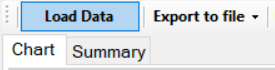
\includegraphics[width=0.3\textwidth]{Graphic/Archive/LoadArchive.png}	
	\caption{Load archive data}
	\label{load_archive_data}
	\end{figure}
	\FloatBarrier

Window \textit{Load data form} possess filter which help us find specific process. Process can be searched by name or date executed

	\begin{figure}[!h] 
	\centering 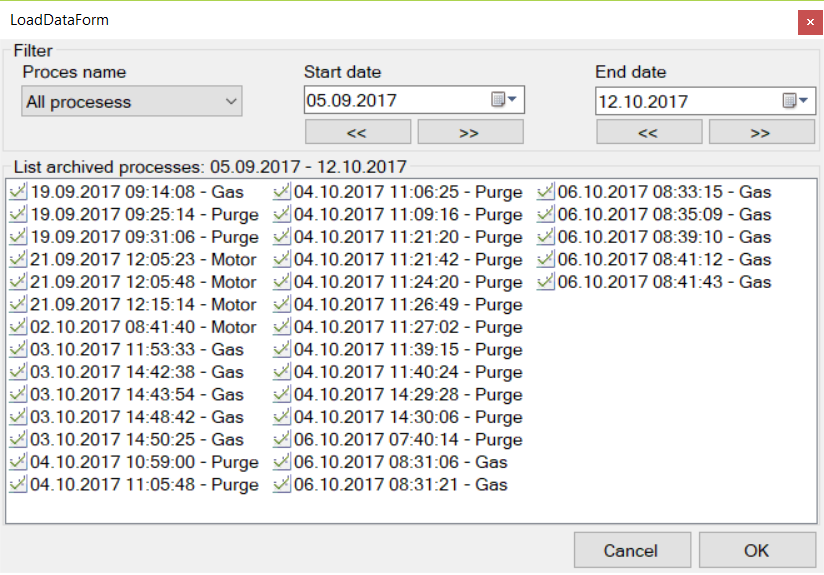
\includegraphics[width=0.8\textwidth]{Graphic/Archive/LoadData.png}	
	\caption{Load archive data}
	\label{load_archive_data}
	\end{figure}
	\FloatBarrier

After select determine process, section \textit{Chart} and \textit{Summary} will be fill of data.\\\\
\textit{Chart} displays selected data of process as a plot
	
\begin{figure}[!h] 
	\centering 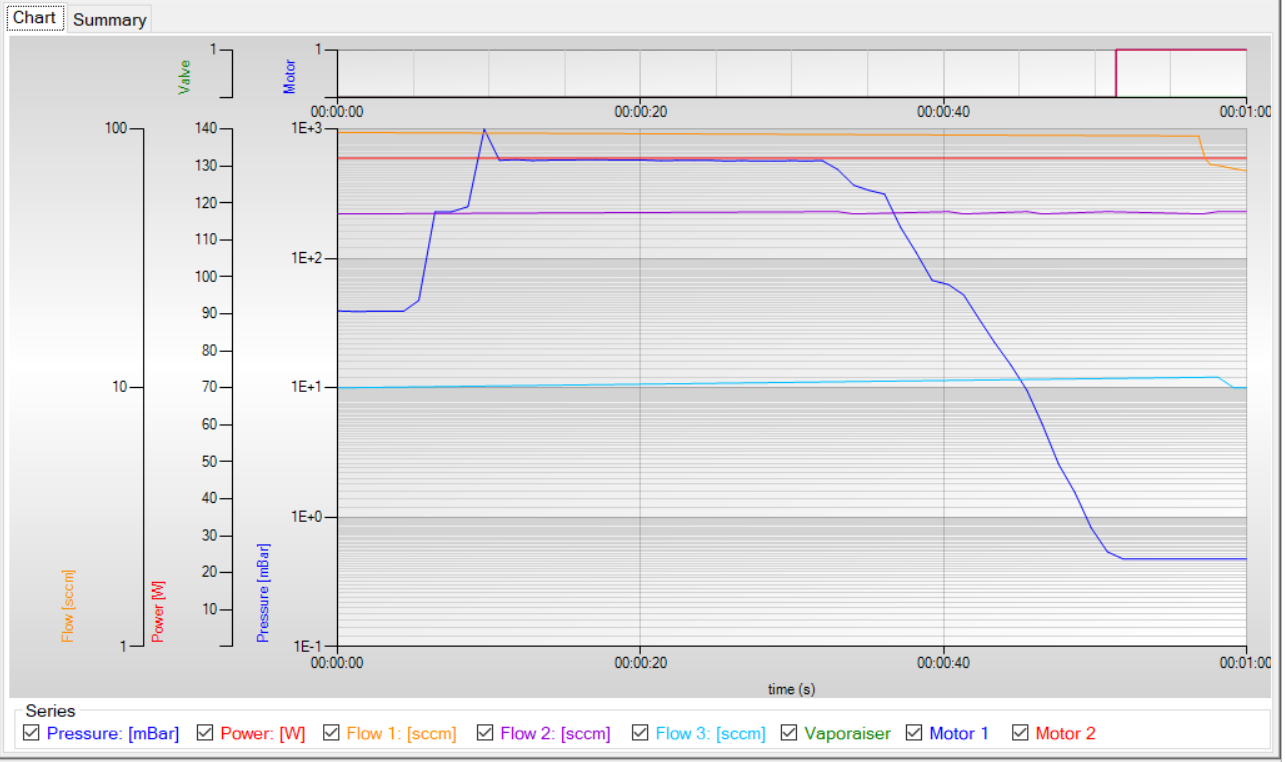
\includegraphics[width=0.8\textwidth]{Graphic/Archive/Chart.png}	
	\caption{Archive chart data}
	\label{archive_chart_data}
	\end{figure}
	\FloatBarrier

\textit{Summary} section contains global view information about process. Information included in section shows:

\begin{itemize}
	\item program information
	\item user which executed process
	\item data executed of process
	\item parameters of subprograms
\end{itemize}

\begin{figure}[!h] 
	\centering 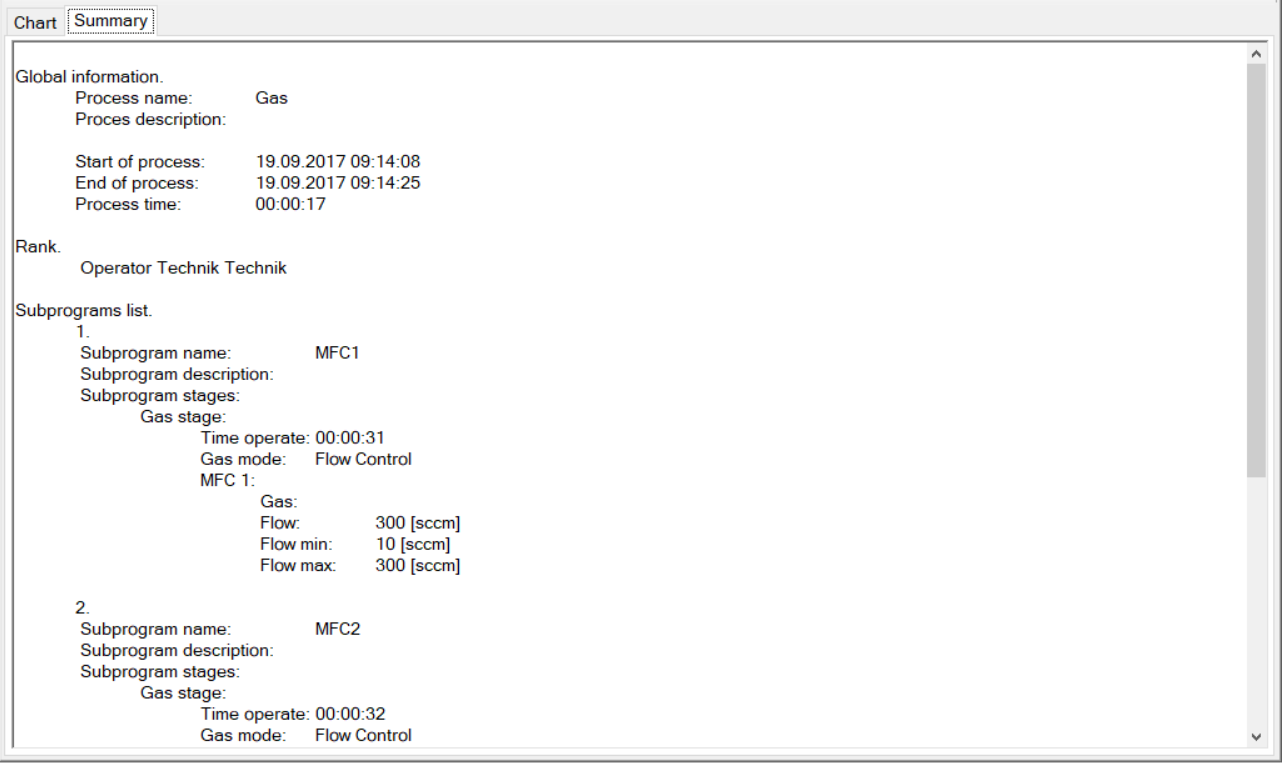
\includegraphics[width=0.8\textwidth]{Graphic/Archive/Summary.png}	
	\caption{Archive summary}
	\label{archive_summary}
	\end{figure}
	\FloatBarrier

Loaded archive data could be exported to one of files:
\begin{itemize}
\item \textit{PDF} 
\item \textit{CSV}
\end{itemize} 

\begin{figure}[!h] 
	\centering 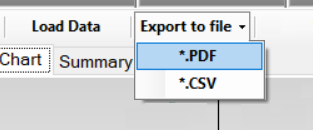
\includegraphics[width=0.4\textwidth]{Graphic/Archive/Export.png}	
	\caption{Archive export data}
	\label{archive_export_data}
	\end{figure}
	\FloatBarrier
